\documentclass{article}

% --- Packages ---
\usepackage[margin=1in]{geometry}
\usepackage{graphicx}
\usepackage{amsmath}
\usepackage{float}
\usepackage{fancyhdr}
\usepackage[hidelinks]{hyperref}
\usepackage{listings}
\usepackage{xcolor}
\usepackage{caption}
\usepackage{subcaption}
\usepackage{booktabs}
\usepackage[T1]{fontenc}
\usepackage[utf8]{inputenc}

% --- Paragraph formatting ---
\setlength{\parindent}{0pt}
\setlength{\parskip}{1em}

% --- Header/Footer ---
\pagestyle{fancy}
\fancyhf{}
\fancyhead[L]{CPU Design Lab Report}
\fancyhead[R]{\thepage}
\renewcommand{\headrulewidth}{0.4pt}

% --- Code listing style (Verilog) ---
\lstdefinelanguage{Verilog}{
    keywords={module, endmodule, input, output, reg, wire, always, begin, end,
              if, else, case, endcase, assign, posedge, negedge, parameter,
              initial},
    keywordstyle=\color{blue}\bfseries,
    comment=[l]{//},
    morecomment=[s]{/*}{*/},
    commentstyle=\color{gray}\itshape,
    stringstyle=\color{red},
    morestring=[b]"
}
\lstset{
    language=Verilog,
    basicstyle=\ttfamily\small,
    breaklines=true,
    frame=single,
    numbers=left,
    numberstyle=\tiny\color{gray},
    tabsize=4,
    showstringspaces=false,
    captionpos=b
}

% -------------------------------------------------------------------------
%                         CUSTOM TITLE PAGE
% -------------------------------------------------------------------------

\title{
    \vspace{1cm}
    \begin{center}
        
\includegraphics[width=6cm]{logo.png}
    \end{center}
    \vspace{1.5cm}
    \Huge\textbf{CPU Design Lab Report}\\
    \vspace{1cm}
    {\LARGE\bfseries Digital Logic Design and Applications}\\
}

\author{
    \LARGE\bfseries Kartike Sharan \quad (2024190595001)\\[0.4em]
    \LARGE\bfseries Instructor: Bo Yan\\[0.4em]
    \Large\bfseries Glasgow College, UESTC\\[0.4em]
    \Large\bfseries Date Performed: 22, 04, 2026
}

\date{}

% -------------------------------------------------------------------------

\begin{document}

\maketitle
\thispagestyle{empty}
\newpage

% =========================================================================
%   SECTION 1 - LAB DESCRIPTION
% =========================================================================

\section{Lab Description}

\textbf{Laboratory Location}

Room 237 in Scientific Research Building (B-Zone), Qingshuihe Campus.

\textbf{Lab Hours}

4 Classes (3 Hours) $\times$ 5

% =========================================================================
%   SECTION 2 - SPECIFICATION
% =========================================================================

\section{Specification}

\subsection{Instruction Set Design}

The CPU's ALU supports 7 operations selected by a 3-bit function code \texttt{alu\_func[2:0]}. Operand A (\texttt{alu\_a}) is always sourced from the destination register \texttt{rd\_q}; operand B (\texttt{alu\_b}) is either the zero-extended immediate offset or the source register \texttt{rs\_q}, selected by \texttt{alu\_in\_sel}. The operations are defined in Table~\ref{tab:isa}.

\begin{table}[H]
    \centering
    \begin{tabular}{cll}
        \toprule
        \textbf{\texttt{alu\_func[2:0]}} & \textbf{Operation} & \textbf{Description} \\
        \midrule
        \texttt{000} & Transfer B  & Output equals operand B (pass-through) \\
        \texttt{001} & ADD         & Addition: $A + B$ \\
        \texttt{010} & SUB         & Subtraction: $A - B$ \\
        \texttt{011} & AND         & Bitwise AND: $A\ \&\ B$ \\
        \texttt{100} & OR          & Bitwise OR: $A\ |\ B$ \\
        \texttt{101} & Left Shift  & Logical shift left by 1 bit: $A \ll 1$ \\
        \texttt{110} & Right Shift & Logical shift right by 1 bit: $A \gg 1$ \\
        \bottomrule
    \end{tabular}
    \caption{ALU Instruction Set --- \texttt{alu\_func[2:0]} encoding}
    \label{tab:isa}
\end{table}

\subsection{Working Flow of the CPU Design}

\begin{figure}[H]
    \centering
    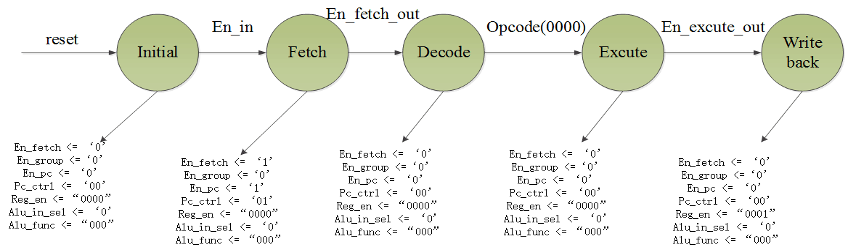
\includegraphics[width=\textwidth,height=7cm,keepaspectratio]{working_flow.png}
    \caption{CPU Working Flow --- FSM State Transition Diagram}
    \label{fig:working_flow}
\end{figure}

% =========================================================================
%   SECTION 3 - ARCHITECTURE DESIGN
% =========================================================================

\section{Architecture Design}

\subsection{Top Level Architecture}

The top-level architecture consists of two primary subsystems: the \texttt{control\_unit} and the \texttt{data\_path}, connected via a set of control and feedback signals. External inputs include the system clock (\texttt{clk}), reset (\texttt{rst}), the 16-bit instruction bus (\texttt{ins[15:0]}), and the RAM output enable (\texttt{en\_ram\_out}). The program counter output (\texttt{pc\_out[15:0]}) drives the RAM address bus (\texttt{addr[15:0]}), and \texttt{en\_ram\_in} controls RAM write enable.

The control unit decodes the instruction register (\texttt{ir\_out[15:0]}) and generates all control signals passed to the datapath, including \texttt{alu\_func[2:0]}, \texttt{alu\_in\_sel}, \texttt{en\_group}, \texttt{en\_pc}, \texttt{pc\_ctrl[1:0]}, \texttt{reg\_en[3:0]}, \texttt{rd[1:0]}, \texttt{rs[1:0]}, and \texttt{offset[7:0]}. The datapath feeds back \texttt{alu\_end} to signal ALU completion.

\subsection{Datapath Unit}

The datapath consists of four submodules: the register file (\texttt{reg\_group}), ALU input multiplexer (\texttt{alu\_mux}), ALU (\texttt{alu}), and program counter (\texttt{pc}).

The \texttt{reg\_group} module contains the CPU registers. It receives the destination register address (\texttt{rd[1:0]}), source register address (\texttt{rs[1:0]}), register write enable (\texttt{reg\_en[3:0]}), and clock, outputting the read data on \texttt{rd\_q[15:0]} and \texttt{rs\_q[15:0]}.

The \texttt{alu\_mux} selects the second ALU operand (\texttt{alu\_b[15:0]}) from one of two sources controlled by \texttt{alu\_in\_sel}: when \texttt{alu\_in\_sel = 0}, \texttt{alu\_b} is assigned the zero-extended 8-bit immediate offset (\texttt{\{8'b0, offset[7:0]\}}); when \texttt{alu\_in\_sel = 1}, \texttt{alu\_b} is assigned the source register output (\texttt{rs\_q[15:0]}). The first ALU operand \texttt{alu\_a} is always sourced directly from \texttt{rd\_q}.

The \texttt{alu} takes \texttt{alu\_a[15:0]} (from \texttt{rd\_q}) and \texttt{alu\_b[15:0]}, performs the operation selected by \texttt{alu\_func[2:0]}, and produces \texttt{alu\_out[15:0]}. The \texttt{en\_out} signal feeds back to the control unit as \texttt{alu\_end} to indicate completion.

The \texttt{pc} module manages the program counter, accepting \texttt{offset\_addr[7:0]} and \texttt{pc\_ctrl[1:0]} to support sequential increment and branch operations, outputting the next address on \texttt{pc\_out[15:0]}.

\begin{figure}[H]
    \centering
    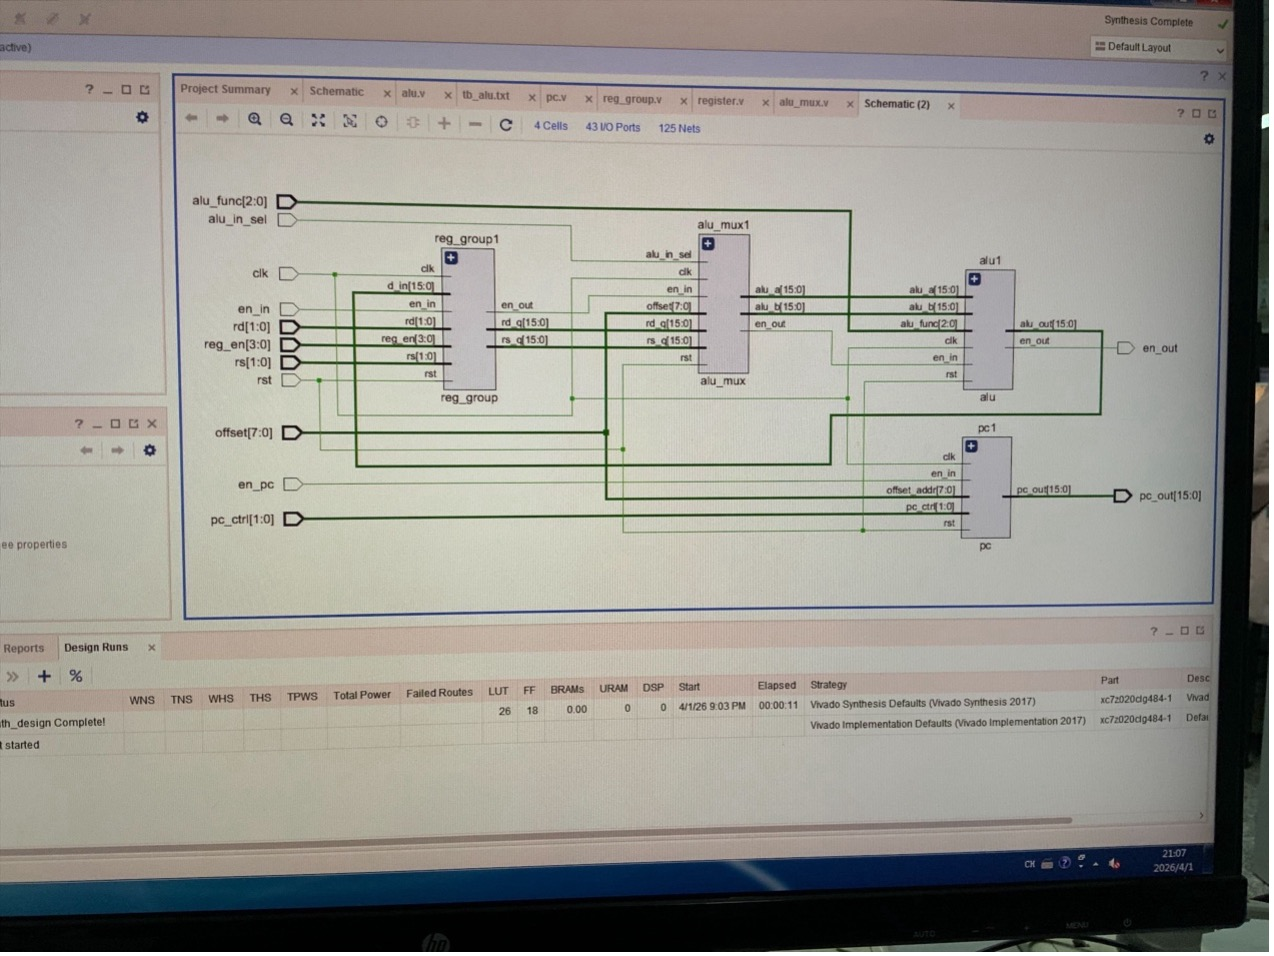
\includegraphics[width=\textwidth,height=7cm,keepaspectratio]{rtl_datapath.png}
    \caption{Datapath Unit --- RTL Schematic}
    \label{fig:datapath}
\end{figure}

\subsection{Control Unit}

The control unit consists of two submodules: the instruction register (\texttt{ir}) and the state transition controller (\texttt{state\_transition}).

The \texttt{ir} module latches the incoming 16-bit instruction from \texttt{ins[15:0]} on each clock edge when \texttt{en\_ram\_out} is asserted, outputting the full instruction word on \texttt{ir\_out[15:0]}. The 16-bit instruction is formatted as: \texttt{opcode[15:12]}, \texttt{rd[11:10]}, \texttt{rs[9:8]}, \texttt{offset[7:0]}. The control unit extracts \texttt{opcode[3:0]} from bits \texttt{[15:12]} and \texttt{rd[1:0]} from bits \texttt{[11:10]} before passing them to the state machine. The \texttt{rs[1:0]} field (bits \texttt{[9:8]}) and \texttt{offset[7:0]} (bits \texttt{[7:0]}) are passed directly to the datapath via \texttt{ir\_out[15:0]}.

The \texttt{state\_transition} module implements the FSM described in Section~2.2. It takes \texttt{alu\_end}, \texttt{clk}, \texttt{rst}, the decoded \texttt{opcode[3:0]} and \texttt{rd[1:0]} fields, and generates all control signals for the datapath: \texttt{alu\_func[2:0]}, \texttt{alu\_in\_sel}, \texttt{en\_fetch}, \texttt{en\_group}, \texttt{en\_pc}, \texttt{pc\_ctrl[1:0]}, and \texttt{reg\_en[3:0]}. The full instruction word \texttt{ir\_out[15:0]} is also passed directly to the datapath for immediate/offset extraction.

\begin{figure}[H]
    \centering
    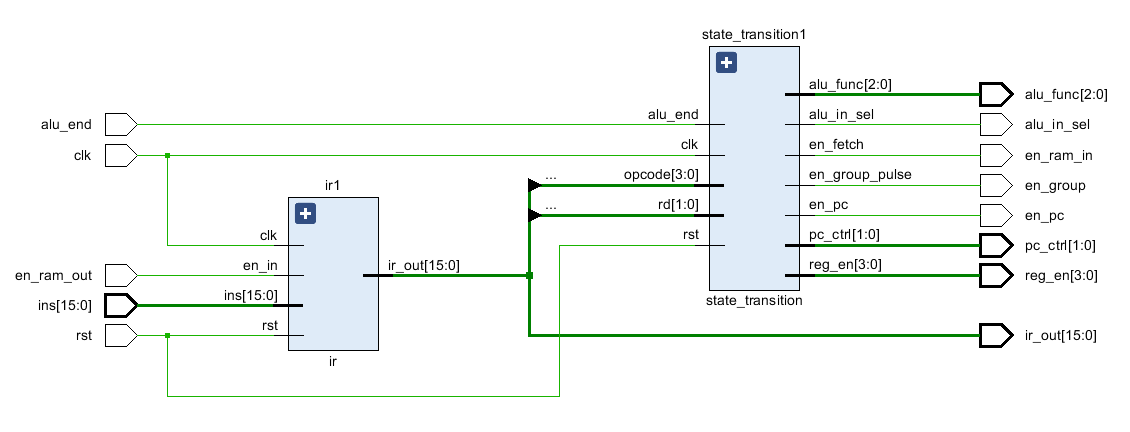
\includegraphics[width=\textwidth,height=7cm,keepaspectratio]{rtl_control.png}
    \caption{Control Unit --- RTL Schematic}
    \label{fig:control}
\end{figure}

% =========================================================================
%   SECTION 4 - IMPLEMENTATION
% =========================================================================

\section{Implementation}

\subsection{Completion Procedures / Code}

\subsubsection{Datapath Unit}

\begin{lstlisting}[caption={Datapath Unit (data\_path.v)}, label={lst:datapath}]
module data_path (
    clk, rst, en_pc, pc_ctrl, offset, en_in, reg_en,
    alu_in_sel, alu_func, en_out, pc_out, rd, rs
);

input clk, rst, en_pc, en_in, alu_in_sel;
input [7:0] offset;
input [1:0] pc_ctrl, rd, rs;
input [3:0] reg_en;
input [2:0] alu_func;
output en_out;
output [15:0] pc_out;

wire en_out_group, en_out_alu_mux;
wire [15:0] rd_q, rs_q, alu_a, alu_b, alu_out;

pc pc1 (
    .clk(clk), .rst(rst), .en_in(en_pc),
    .pc_ctrl(pc_ctrl), .offset_addr(offset), .pc_out(pc_out)
);

reg_group reg_group1 (
    .clk(clk), .rst(rst), .en_in(en_in),
    .reg_en(reg_en), .d_in(alu_out), .rd(rd), .rs(rs),
    .rd_q(rd_q), .rs_q(rs_q), .en_out(en_out_group)
);

alu_mux alu_mux1 (
    .clk(clk), .rst(rst), .en_in(en_out_group),
    .rd_q(rd_q), .rs_q(rs_q), .offset(offset),
    .alu_in_sel(alu_in_sel), .alu_a(alu_a), .alu_b(alu_b),
    .en_out(en_out_alu_mux)
);

alu alu1 (
    .clk(clk), .rst(rst), .en_in(en_out_alu_mux),
    .alu_a(alu_a), .alu_b(alu_b), .alu_func(alu_func),
    .en_out(en_out), .alu_out(alu_out)
);

endmodule
\end{lstlisting}

\subsubsection{Control Unit}

\begin{lstlisting}[caption={Control Unit (control\_unit.v)}, label={lst:control}]
module control_unit (
    clk, rst, alu_end, ins, en_ram_in, en_ram_out,
    en_group, en_pc, reg_en, alu_in_sel, alu_func, pc_ctrl, ir_out
);

input clk, rst, alu_end, en_ram_out;
input [15:0] ins;
output en_ram_in, en_group, en_pc, alu_in_sel;
output [3:0] reg_en;
output [2:0] alu_func;
output [1:0] pc_ctrl;
output [15:0] ir_out;

ir ir1 (
    .clk(clk), .rst(rst), .ins(ins),
    .en_in(en_ram_out), .ir_out(ir_out)
);

state_transition state_transition1 (
    .clk(clk), .rst(rst), .alu_end(alu_end),
    .rd(ir_out[11:10]), .opcode(ir_out[15:12]),
    .en_fetch(en_ram_in), .en_group_pulse(en_group),
    .en_pc(en_pc), .pc_ctrl(pc_ctrl),
    .reg_en(reg_en), .alu_in_sel(alu_in_sel), .alu_func(alu_func)
);

endmodule
\end{lstlisting}

\subsubsection{CPU (Top Level)}

\begin{lstlisting}[caption={CPU Top Level (cpu.v)}, label={lst:cpu}]
module cpu (clk, rst, addr, ins, en_ram_in, en_ram_out);

input clk, rst, en_ram_out;
input [15:0] ins;
output [15:0] addr;
output en_ram_in;

wire en_pc, en_group, alu_in_sel, alu_end;
wire [1:0] pc_ctrl;
wire [3:0] reg_en;
wire [2:0] alu_func;
wire [15:0] ir_out;

data_path data_path1 (
    .clk(clk), .rst(rst), .offset(ir_out[7:0]),
    .en_pc(en_pc), .pc_ctrl(pc_ctrl), .en_in(en_group),
    .reg_en(reg_en), .rd(ir_out[11:10]), .rs(ir_out[9:8]),
    .alu_in_sel(alu_in_sel), .alu_func(alu_func),
    .en_out(alu_end), .pc_out(addr)
);

control_unit control_unit1 (
    .clk(clk), .rst(rst), .alu_end(alu_end),
    .ins(ins), .en_ram_in(en_ram_in), .en_ram_out(en_ram_out),
    .en_group(en_group), .en_pc(en_pc), .reg_en(reg_en),
    .alu_in_sel(alu_in_sel), .alu_func(alu_func),
    .pc_ctrl(pc_ctrl), .ir_out(ir_out)
);

endmodule
\end{lstlisting}

\subsection{RTL Screenshots}

\subsubsection{Datapath Unit}

\begin{figure}[H]
    \centering
    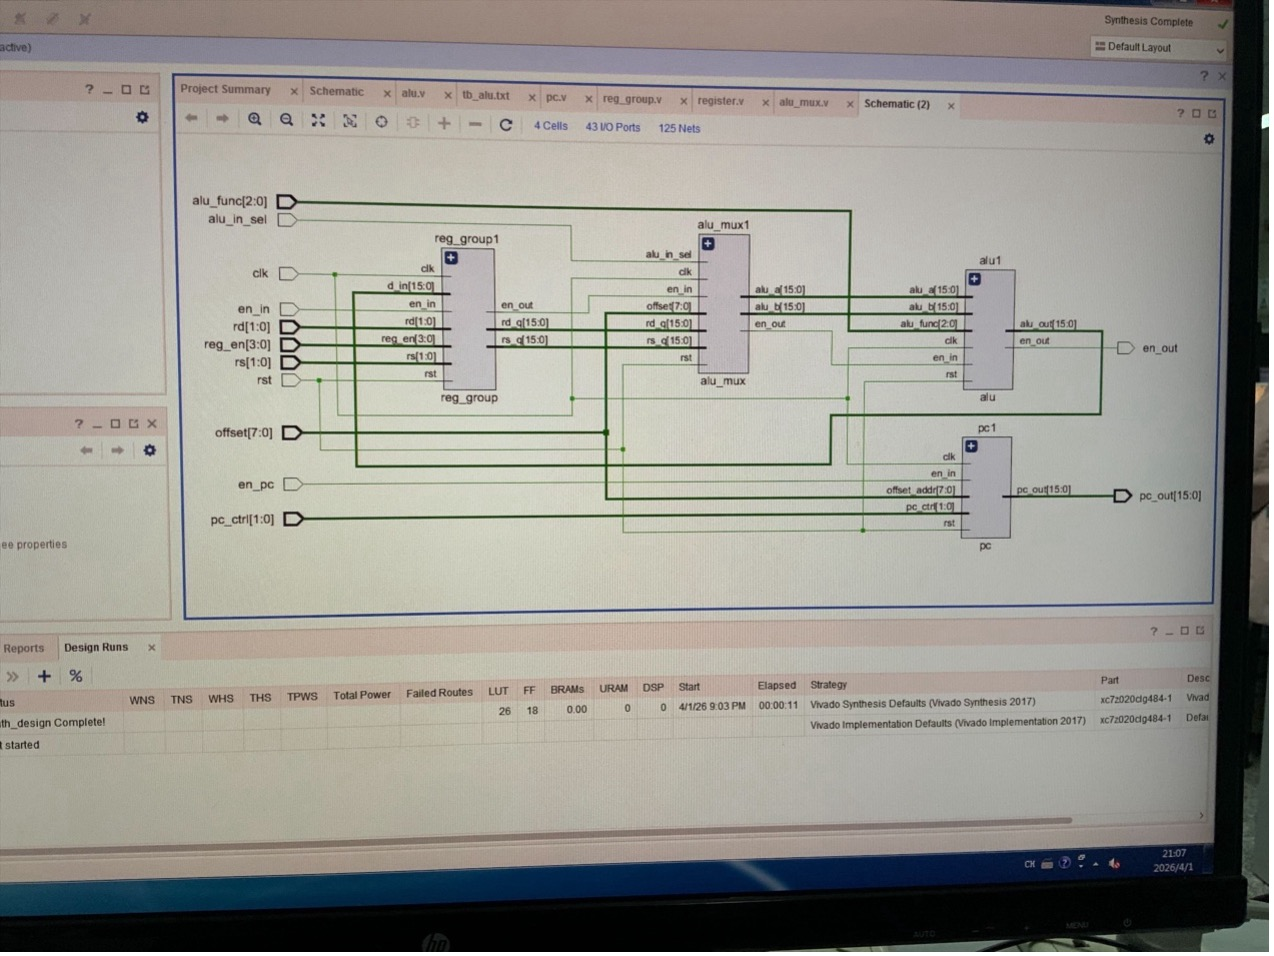
\includegraphics[width=\textwidth,height=7cm,keepaspectratio]{rtl_datapath.png}
    \caption{RTL Schematic --- Datapath Unit}
    \label{fig:rtl_datapath}
\end{figure}

\subsubsection{Control Unit}

\begin{figure}[H]
    \centering
    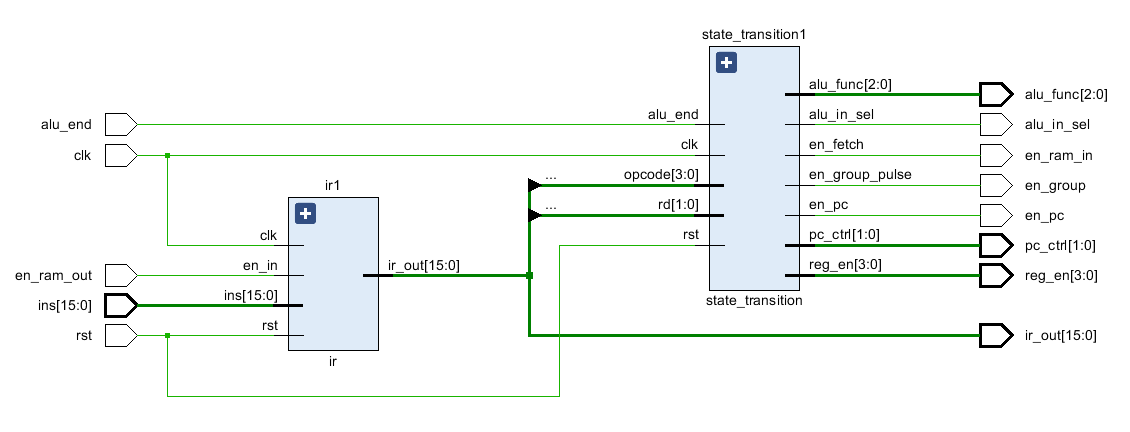
\includegraphics[width=\textwidth,height=7cm,keepaspectratio]{rtl_control.png}
    \caption{RTL Schematic --- Control Unit}
    \label{fig:rtl_control}
\end{figure}

\subsubsection{CPU}

\begin{figure}[H]
    \centering
    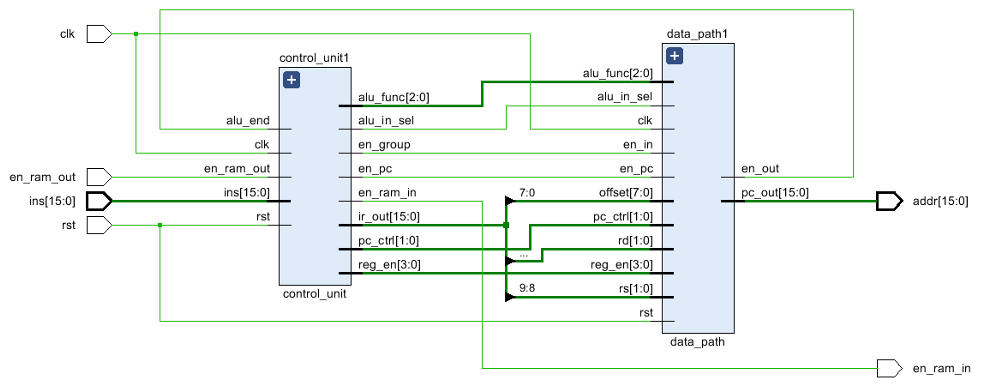
\includegraphics[width=\textwidth,height=7cm,keepaspectratio]{rtl_cpu.png}
    \caption{RTL Schematic --- Full CPU}
    \label{fig:rtl_cpu}
\end{figure}

% =========================================================================
%   SECTION 5 - TESTBENCH AND ANALYSIS
% =========================================================================

\section{Testbench and Analysis}

\subsection{Testbench Code}

\begin{lstlisting}[caption={CPU Testbench (tb\_top\_cpu.v)}, label={lst:tb}]
module tb_top_cpu();

reg clk, rst;
wire [15:0] ins;
wire        en_ram_in;
wire        en_ram_out;
wire [15:0] addr;

parameter Tclk = 10;

cpu test_cpu (
    .clk(clk), .rst(rst),
    .en_ram_in(en_ram_in),
    .en_ram_out(en_ram_out),
    .ins(ins),
    .addr(addr)
);

rom tb_rom (
    .clk(clk), .rst(rst),
    .ready(en_ram_in),
    .addr(addr),
    .dout(ins),
    .en_out(en_ram_out)
);

initial begin
    clk = 1;
    forever #(Tclk/2) clk = ~clk;
end

initial begin
    rst = 0;
    #(Tclk*12) rst = 1;
end

endmodule
\end{lstlisting}

\subsection{Simulation Timing Diagrams}

\subsubsection{Datapath Unit}

\begin{figure}[H]
    \centering
    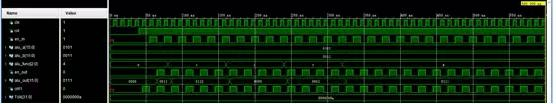
\includegraphics[width=\textwidth,height=7cm,keepaspectratio]{sim_datapath.jpeg}
    \caption{Datapath Unit --- Simulation Timing Diagram}
    \label{fig:sim_datapath}
\end{figure}

\subsubsection{Control Unit}

\begin{figure}[H]
    \centering
    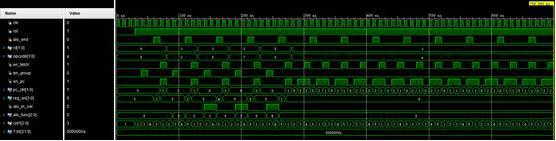
\includegraphics[width=\textwidth,height=7cm,keepaspectratio]{sim_control.jpeg}
    \caption{Control Unit --- Simulation Timing Diagram}
    \label{fig:sim_control}
\end{figure}

\subsubsection{CPU (Full Integration)}

\begin{figure}[H]
    \centering
    \includegraphics[width=\textwidth,height=7cm,keepaspectratio]{sim_cpu.jpeg}
    \caption{Full CPU --- Simulation Timing Diagram}
    \label{fig:sim_cpu}
\end{figure}

\subsection{Analysis}

The testbench instantiates the \texttt{cpu} and \texttt{rom} modules together to simulate the full CPU pipeline. The clock period is set to \texttt{Tclk = 10ns} and reset is held low for 12 clock cycles to ensure all registers and the FSM initialise cleanly before execution begins.

The ROM is preloaded with 11 instructions that exercise all implemented opcodes. The execution trace is shown in Table~\ref{tab:rom_trace}. Note that the ADD instruction (\texttt{opcode = 0010}) is implemented with \texttt{alu\_in\_sel = 0} in the state transition module, meaning \texttt{alu\_b} is sourced from the zero-extended immediate offset field. For instructions where \texttt{offset = 0}, the ADD operation computes \texttt{rd = rd + 0}. The results column reflects the actual simulated behaviour.

\begin{table}[H]
    \centering
    \begin{tabular}{clll}
        \toprule
        \textbf{Addr} & \textbf{Instruction} & \textbf{Operation} & \textbf{Simulated Result} \\
        \midrule
        0  & MOVEB R1, \#1     & R1 $\leftarrow$ offset(1)  & R1 = 1 \\
        1  & MOVEB R2, \#2     & R2 $\leftarrow$ offset(2)  & R2 = 2 \\
        2  & MOVEB R3, \#8     & R3 $\leftarrow$ offset(8)  & R3 = 8 \\
        3  & ADD R0, offset(0) & R0 $\leftarrow$ R0 + 0     & R0 = 0 \\
        4  & ADD R0, offset(0) & R0 $\leftarrow$ R0 + 0     & R0 = 0 \\
        5  & MOVEB R1, \#8     & R1 $\leftarrow$ offset(8)  & R1 = 8 \\
        6  & SUB R1, R0        & R1 $\leftarrow$ R1 - R0    & R1 = 8 \\
        7  & OR R1, R0         & R1 $\leftarrow$ R1 $|$ R0  & R1 = 8 \\
        8  & MOVEB R2, \#1     & R2 $\leftarrow$ offset(1)  & R2 = 1 \\
        9  & ADD R1, offset(0) & R1 $\leftarrow$ R1 + 0     & R1 = 8 \\
        10 & JUMP 10           & PC $\leftarrow$ 10         & Halt   \\
        \bottomrule
    \end{tabular}
    \caption{ROM Test Program --- Execution Trace}
    \label{tab:rom_trace}
\end{table}

The CPU correctly sequences through the Initial, Fetch, Decode, Execute, and Write Back states for each instruction. The \texttt{alu\_end} feedback signal ensures the FSM waits for ALU completion before advancing to Write Back. The JUMP instruction bypasses the ALU pipeline and directly updates the PC via \texttt{pc\_ctrl = 2'b10}, causing the CPU to loop at address 10.

It should be noted that the ADD instruction (\texttt{opcode = 0010}) in the \texttt{state\_transition} module is implemented with \texttt{alu\_in\_sel = 0}, meaning \texttt{alu\_b} is always sourced from the zero-extended offset field rather than the source register \texttt{rs\_q}. Since the ADD instructions in the ROM have \texttt{offset = 0}, these instructions effectively compute \texttt{rd + 0}, leaving the destination register unchanged. As a result, \texttt{R0} remains 0 throughout, and the SUB and OR operations produce \texttt{R1 = 8 - 0 = 8} and \texttt{R1 = 8 | 0 = 8} respectively.

% =========================================================================
%   SECTION 6 - SUGGESTIONS
% =========================================================================

\section{Your Suggestions for This Lab / Course}

This lab provided a comprehensive introduction to CPU design, covering the full implementation flow from instruction set specification through RTL coding, synthesis, and simulation. Designing the FSM-based control unit and connecting it to the datapath reinforced the relationship between hardware description and actual circuit behaviour.

One suggestion would be to include a brief guided walkthrough of the ILA (Integrated Logic Analyser) setup in Vivado, as monitoring internal signals on the FPGA board requires creating the ILA IP core which is not immediately obvious for first-time users.

Overall the lab was well structured and the progressive build-up from individual modules to the full CPU made the complexity manageable.

\end{document}